% flashcards-title: Square meter with one centimeter square marked in a corner
% flashcards-desc: A large square with each side marked as one meter, equal to one hundred centimeters. Near the bottom left corner a tiny shaded square is drawn with a note marking it as one centimeter by one centimeter, deliberately not to scale, and faint grid lines fade out along the bottom edge and left edge.
\documentclass[dvisvgm,tikz,border=8pt]{standalone}
\usepackage{tikz}
\usetikzlibrary{arrows.meta,calc,positioning}
\definecolor{DeckInk}{HTML}{172A3A}
\definecolor{DeckAccent}{HTML}{176B87}
\definecolor{DeckWarm}{HTML}{D97706}
\definecolor{DeckMuted}{HTML}{667784}
\definecolor{DeckPaper}{HTML}{F7FAFC}
\tikzset{
  every node/.style={font=\sffamily, text=DeckInk},
  object/.style={draw=DeckInk, line width=1.1pt, fill=DeckPaper},
  primary/.style={draw=DeckAccent, line width=1.5pt},
  boundary/.style={draw=DeckAccent, line width=1.5pt, dashed, rounded corners=6pt},
  guide/.style={draw=DeckMuted, line width=0.9pt, dashed},
  dimension/.style={{Stealth[length=3.2mm,width=2.2mm]}-{Stealth[length=3.2mm,width=2.2mm]}, draw=DeckWarm, line width=1.2pt},
  motion/.style={-{Stealth[length=3.5mm,width=2.5mm]}, draw=DeckAccent, line width=1.5pt, dashed},
}

\begin{document}
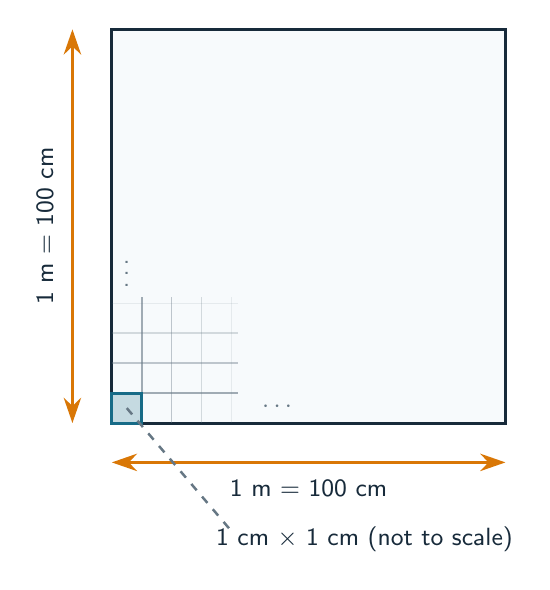
\begin{tikzpicture}[x=1cm,y=1cm]
  % Big square
  \draw[object] (0,0) rectangle (5,5);
  % Faint grid lines fading out from the bottom-left corner
  \foreach \i/\o in {0.38/60, 0.76/40, 1.14/25, 1.52/12}
    \draw[DeckMuted, line width=0.6pt, opacity={\o/100}] (\i,0) -- (\i,1.6);
  \foreach \j/\o in {0.38/60, 0.76/40, 1.14/25, 1.52/12}
    \draw[DeckMuted, line width=0.6pt, opacity={\o/100}] (0,\j) -- (1.6,\j);
  \node[font=\sffamily\small, text=DeckMuted] at (2.1,0.2) {$\cdots$};
  \node[font=\sffamily\small, text=DeckMuted] at (0.19,2.0) {$\vdots$};
  % Exaggerated unit square in the corner
  \fill[DeckAccent!25] (0,0) rectangle (0.38,0.38);
  \draw[DeckAccent, line width=1.1pt] (0,0) rectangle (0.38,0.38);
  % Dimension arrows
  \draw[dimension] (0,-0.5) -- (5,-0.5);
  \node[below, font=\sffamily\small] at (2.5,-0.6) {1 m $=$ 100 cm};
  \draw[dimension] (-0.5,0) -- (-0.5,5);
  \node[left, font=\sffamily\small, rotate=90, anchor=south] at (-0.62,2.5) {1 m $=$ 100 cm};
  % Unit-square note
  \draw[guide] (0.19,0.19) -- (1.5,-1.35);
  \node[below right, font=\sffamily\small, align=left] at (1.2,-1.20) {1 cm $\times$ 1 cm (not to scale)};
\end{tikzpicture}
\end{document}
